\documentclass{../knittingpattern}

\usepackage{amssymb}
\usepackage{amsmath}
\usepackage{tikz}
\usetikzlibrary{matrix,arrows,shapes,positioning,fit,calc,decorations.pathmorphing,decorations.pathreplacing,fadings}
\tikzstyle{every picture} += [remember picture]

\newcommand{\K}{\blacksquare}
\renewcommand{\P}{\square}


% Knitting Pattern Commands
% \intro{Text}{pic}
% \note{borderColour}{backgroundColour}{Title}{Text}
% \diagram{diag}
% \begin{pattern}{colour1}{colour2} Col & (st) \end{pattern}
% \important{borderColour}{backgroundColour}{Text}
% \biog{pic}{Text}
% \cpyrght{Name}

\definecolor{colour0}{HTML}{437399}
\definecolor{colour1}{HTML}{FFFFFF}
\definecolor{colour2}{HTML}{68B4EF}
\definecolor{colour3}{HTML}{8FCFEF}
\definecolor{colour4}{HTML}{CADFEF}
\definecolor{colour5}{HTML}{D7E5EF}
\definecolor{colour6}{HTML}{F0F7FC}

\usepackage{graphicx}
\graphicspath{{../images/}}

\newcommand{\ccbysa}{\raisebox{-0.5\height}{\includegraphics[height=16pt]{cc.pdf}\includegraphics[height=16pt]{by.pdf}\includegraphics[height=16pt]{sa.pdf}}}
%\newcommand{\ccbysa}{\raisebox{-0.5\height}{\includegraphics[height=18pt]{by-sa.pdf}}}


\begin{document}

\title{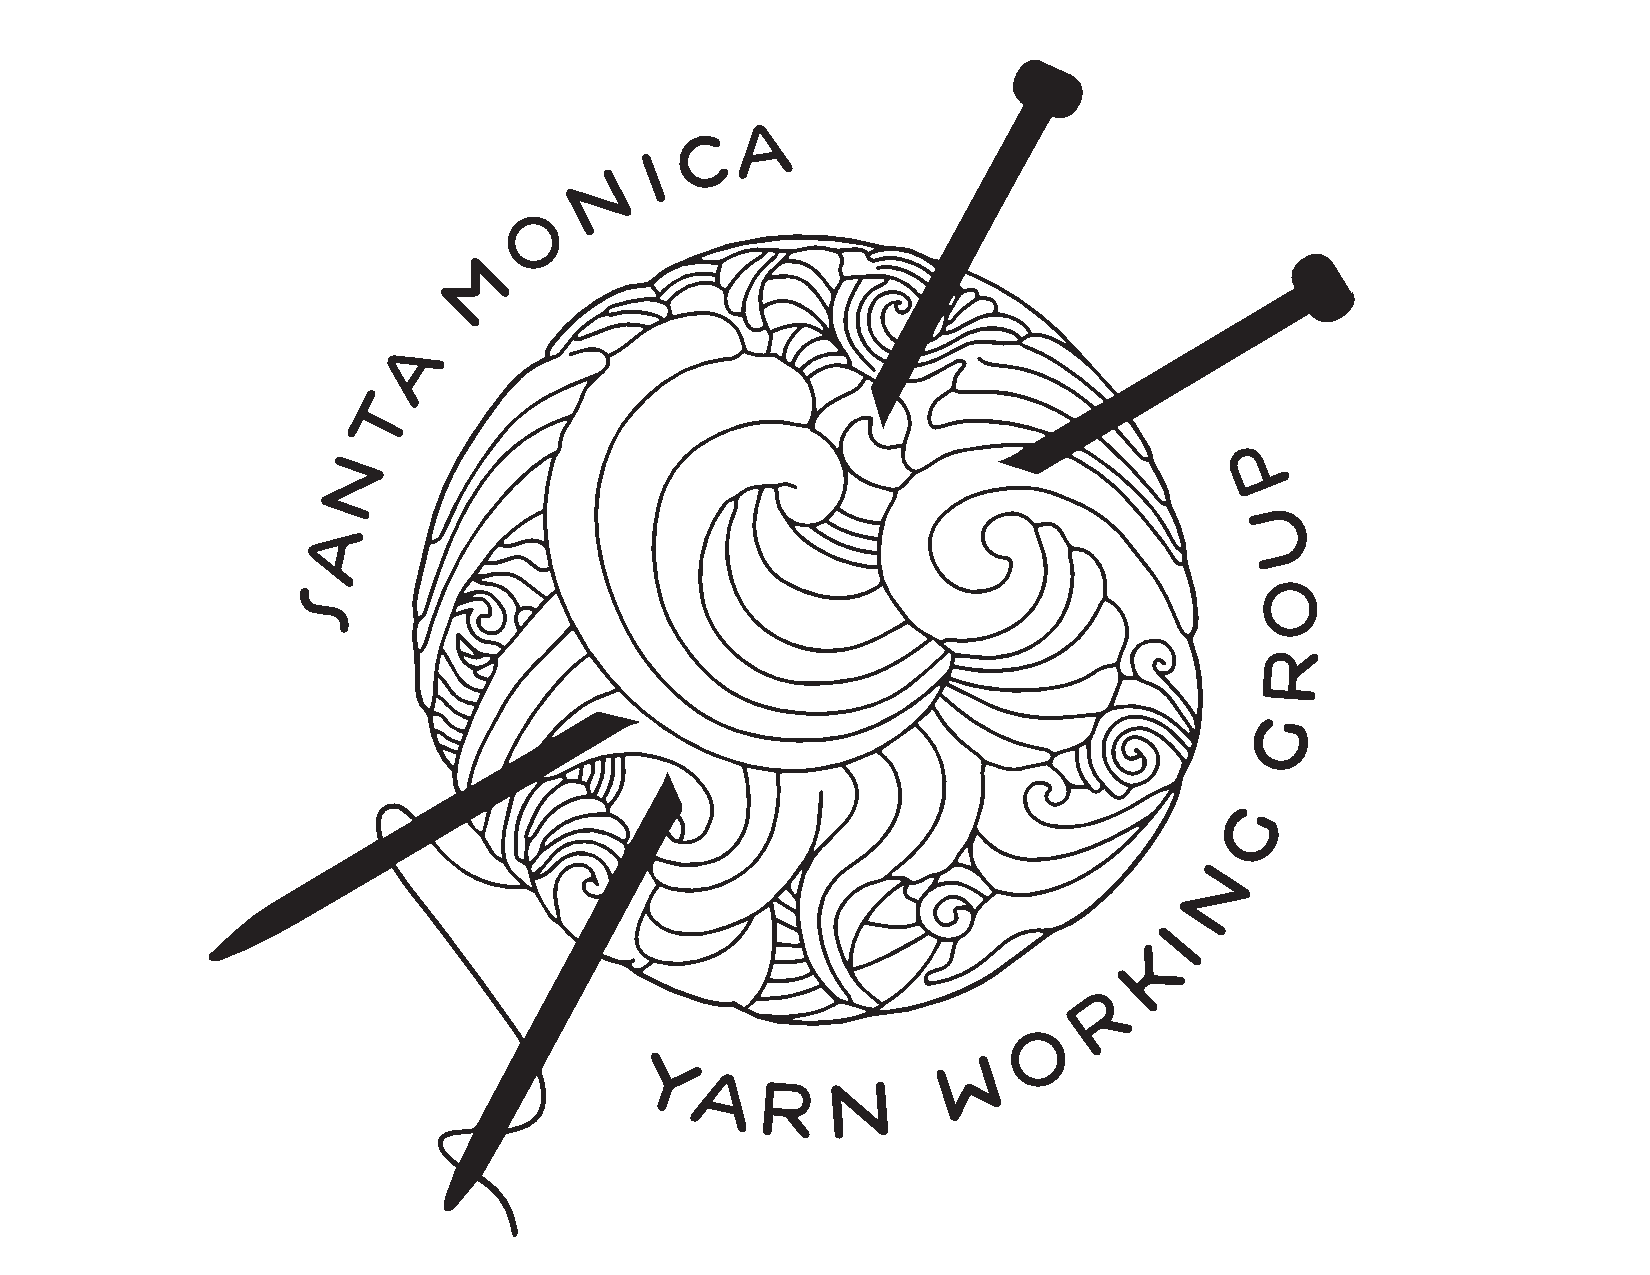
\includegraphics[width=4.5cm]{SMYWG_logo.pdf}\\\textcolor{colour0}{\bf Double Knit Cellular Automaton Scarf}}
\author{Nigel Stepp}
\date{}
\maketitle

%\cpyrght{\copyright 2019 Santa Monica Yarn Working Group, Santa Monica, Ca \hfill \cc\ccby\ccsa}
\cpyrght{\copyright 2019 Santa Monica Yarn Working Group, Santa Monica, Ca \hfill \ccbysa}

\intro{

This pattern combines the \emph{double knitting} yarn working technique with a computational construct known as \emph{elementary cellular automata}. It turns out that these two concepts have a natural affinity for each other that translates to fun, beautiful, and unique craft projects.

We will begin by introducing elementary cellular automata in the context of knitting, then show how extending the technique to double knitting results in an even more elegant and natural combination of yarn craft and mathematics.

Lastly, the method will be applied to create a double-knit scarf.

}{rule90.png}


\section*{Elementary Cellular Automata}
Elementary cellular automata (ECA) are systems consisting of a collection of cells (or a row of stitches) that are either \emph{on} or \emph{off}, along with a rule for how to update the cells (how to work the next row). Consider a row of 5 stitches like the following, where $\K$ = CC and $\P$ = MC.

\[
\begin{matrix}
\K & \P & \K & \K & \P \\
\end{matrix}
\]

In terms of cellular automata, this is a 1 dimensional grid of 5 cells. For us, it's a row with 5 stitches. In order to know how to work the next row, we look to the previous row and apply a rule. Specifically, we look in the previous row to the stitches left and right of the current stitch.

\begin{figure}[h]
\begin{center}
\raisebox{-0.5\height}{\includegraphics[scale=0.4]{knit-2color.png}}
\hspace{3em}
\raisebox{-0.5\height}{
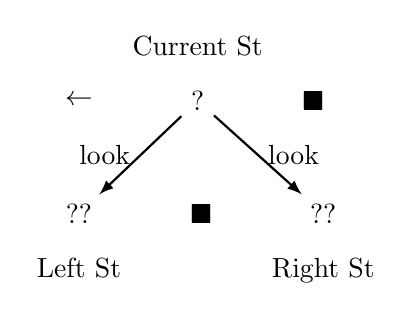
\begin{tikzpicture}

\node (r1s1) {??};
\node[right=of r1s1] (r1s2) {$\blacksquare$};
\node[right=of r1s2] (r1s3) {??};

\node[above=of r1s1] (r2s1) {$\leftarrow$};
\node[right=of r2s1] (r2s2) {?};
\node[right=of r2s2] (r2s3) {$\blacksquare$};

\draw[thick,-latex] (r2s2) -- node[left] {look} (r1s1);
\draw[thick,-latex] (r2s2) -- node[right] {look} (r1s3);

\node[below=0.2cm of r1s1] {Left St};
\node[below=0.2cm of r1s3] {Right St};
\node[above=0.2cm of r2s2] {Current St};

\end{tikzpicture}
}
\end{center}

\caption{\label{fig:left-right-stitch}(left) The left stitch is still on the needle, while the right stitch has been passed by. (right) Schematic of left and right stitches relative to the current stitch. The small arrow shows direction of work on the current row. Image Credit: Joni Coniglio/Potter Craft, 2011}
\end{figure}

There are many possible rules, each one determining what to do given a particular combination of left and right stitch. One such rule is: If the left and right stitches are the same, use MC, if they are different, use CC. This rule produced the image in the upper-right, and is summarized in table \ref{tab:rule90} below.


\begin{table}[h]
\begin{center}
\begin{tabular}{cc}
\hline
Left,Right & Result \\
\hline
$\P,\P$ & $\P$ \\
$\K,\K$ & $\P$ \\
$\P,\K$ & $\K$ \\
$\K,\P$ & $\K$ \\
\hline
\end{tabular}
\caption{\label{tab:rule90}A rule consists of a mapping from combinations of $\K$ and $\P$ to either $\K$ or $\P$. This rule demonstrates ECA ``rule 90", or the ``exclusive or" (XOR) rule.}
\end{center}
\end{table}


Using the rule in table \ref{tab:rule90}, here are 5 rows worked top-down starting with the initial row from above:
\[
\begin{matrix}
1 & \K & \P & \K & \K & \P \\
2 & \P & \P & \K & \K & \P \\
3 & \P & \K & \K & \K & \K \\
4 & \P & \K & \P & \P & \K \\
5 & \P & \P & \K & \K & \P \\
\end{matrix}
\]

Note that ``left" and ``right" for the first and last stitches in a row are special. We treat the row as if it makes a circle, with the first and last stitches next to each other. What this means is that when you are working the first or last stitch of a row and the stitch you want to look at isn't there, go to the other side of the previous row to look at the first or last stitch on that side.

Since this can be confusing the first few times around, below is a diagram showing just two rows with arrows pointing to the stitches that resulted in the choice for the second row.

\begin{center}
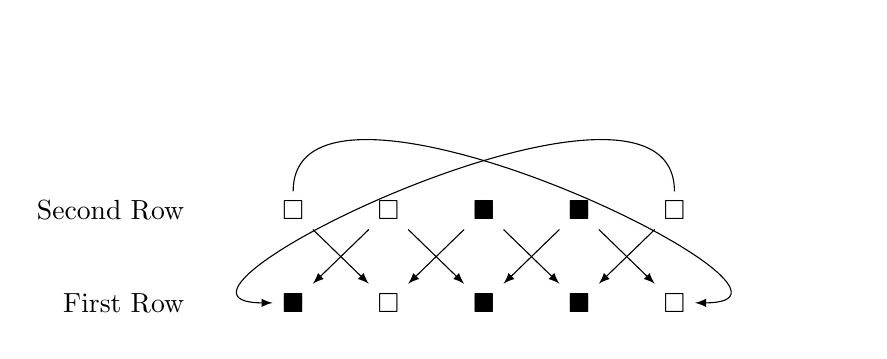
\begin{tikzpicture}

\matrix (m) [matrix of math nodes, row sep=2em, column sep=2em] {
\P & \P & \K & \K & \P \\
\K & \P & \K & \K & \P \\
};

\draw[-latex] (m-1-1) edge[out=90,in=0] (m-2-5);
\draw[-latex] (m-1-1) edge (m-2-2);

\draw[-latex] (m-1-2) edge (m-2-1);
\draw[-latex] (m-1-2) edge (m-2-3);

\draw[-latex] (m-1-3) edge (m-2-2);
\draw[-latex] (m-1-3) edge (m-2-4);

\draw[-latex] (m-1-4) edge (m-2-3);
\draw[-latex] (m-1-4) edge (m-2-5);

\draw[-latex] (m-1-5) edge (m-2-4);
\draw[-latex] (m-1-5) edge[out=90,in=180] (m-2-1);

\node[left=of m-2-1] {First Row};
\node[left=of m-1-1] {Second Row};

\end{tikzpicture}
\end{center}

\section*{ECA and Double Knitting}


Double knitting (DK) is a relatively standard yarn working technique in which two separate yarns are knit and purled in alternation so that two opposing sheets of stockinette are created. Knowledge of this technique will be assumed below, and only explained when needed to illustrate a link to ECA.

\begin{figure}[h]
\label{fig:double-knitting}
\begin{center}
\includegraphics[scale=0.4]{doubleknit.png}
\end{center}

\caption{Adapted from fig.~\ref{fig:left-right-stitch}, each double-knit stitch comes in MC-CC pairs. Position of the ``right" stitch remains the same, while the ``left" stitch is now farther down the needle. The two loops closest to the end are part of the same double-knit stitch. The loop marked Left St in the figure was purled on the opposite side, so will show on this side as a knit stitch. Therefore, that is the loop we wish to compare to the Right St, which is also a knit.}
\end{figure}


A defining feature of DK is that for each double-knit stitch, one yarn is knit, while the other is purled. Whichever yarn is knit will show on the same side, while the purl stitch will show as a knit stitch on the opposite side. Thus, one can switch between visible yarns quite easily by changing which yarn is knit. In terms of MC and CC, we say that typically MC is knit and CC is purled. To create a pattern, the CC is brought to the front by knitting CC and purling MC, switching the usual order. The colors are automatically reversed on the opposite side.

Since the knits and purls in DK \emph{always} come in pairs, we can refer to only the knit stitch and leave the purl stitch to be assumed. This convention allows direct application of the CA discussion above. If MC is required, knit MC (and purl CC), otherwise knit CC (and purl MC). The knit-purl alternation of the DK technique never changes, only \emph{which} yarn is knit or purled.

The combination of DK and ECA adds elegance to both the yarn-crafted work and the mathematical underpinning. With many color changes, other techniques of changing yarn color would leave a wrong side with many carried yarns or woven-in ends. DK allows seamless color change, even if alternating colors every stitch.

On the mathematical side, DK allows for a more direct mapping between ECA and yarn working. As initially described, knitting an ECA pattern specifies whether to use an MC or CC yarn to work the next stitch. While that still applies to DK (along with the assumed purl stitch), we may also formulate in terms of swapping the knit-purl yarn order or not. \emph{Swapped} or \emph{not swapped} is a natural boolean state, which is the same domain used for ECA; a ``cell" is either \emph{on} or \emph{off}, or in terms of bits, 1 or 0. As such, the mapping from ECA to DK is simply a map from 1 and 0 to \emph{swapped} and \emph{not swapped}. Indeed, that is the \emph{only} mapping required to equate ECA and DK. Spoken mathematically, 1-dimensional elementary cellular automata is isomorphic to double knitting with bits defined by \emph{swapped} or \emph{not swapped} yarn order.

A direct mapping between ECA and DK means that every ECA pattern is also a double-knit yarn working pattern. Likewise, the initial requirements for both are the same: a number of cells, an initial state for the cells, and an update rule. 

\newpage
\section*{ECA-DK Scarf}

\note{colour2}{colour1}{Materials}{
\begin{tabular}{ll}
2 skeins MC & US 10 (6.5mm) needles \\
2 skeins CC & \\
\end{tabular}
}

\note{colour1}{colour6}{Abbreviations}{
\begin{tabular}{ll}
MC, CC & Main Color, Contrast Color\\
k, p & Knit, Purl\\
pbl & Purl through the back loop\\
\end{tabular}
}

\subsection*{Number of Cells and Initial State}

Choose a seed of 40 0s or 1s. I chose the ascii bit string corresponding to ``hbrew", or 0110 1000 0110 0010 0111 0010 0110 0101 0111 0111.

\begin{pattern}{colour1}{colour6}
long tail cast on with CC & 40 st\\
k CC, pbl MC & to end\\
for each position in seed, k1p1; k in MC for 0, k in CC for 1 & to end\\
\end{pattern}


\subsection*{Appication of ECA Rule}

Rule Table:
\begin{center}
\begin{tabular}{cc}
\hline
Left,Right & Result \\
\hline
$\P,\P$ & $\P$ \\
$\K,\K$ & $\P$ \\
$\P,\K$ & $\K$ \\
$\K,\P$ & $\K$ \\
\hline
\end{tabular}
\end{center}

\begin{pattern}{colour1}{colour6}
k1p1; k in MC or CC according to the Rule Table & to end\\
swap MC and CC in alternating rows & \\
\end{pattern}



\newpage
\section*{An ECA-DK Meta-Pattern}


Applying the mapping from above, it is possible to create a meta-pattern, or template, which can be used to turn any instance of ECA into a yarn working pattern:


\note{colour2}{colour1}{Materials}{
\begin{tabular}{ll}
$X$ skeins MC & US $Y$ ($y$mm) needles \\
$X$ skeins CC & \\
\end{tabular}
}

\note{colour1}{colour6}{Abbreviations}{
\begin{tabular}{ll}
MC, CC & Main Color, Contrast Color\\
k, p & Knit, Purl\\
pbl & Purl through the back loop\\
\end{tabular}
}

\subsection*{Number of Cells and Initial State}

Choose a string of 0 and 1, $N$ elements long. This seed will be the initial state. For instance, with $N=5$, a seed could be 10110.

\begin{pattern}{colour6}{colour1}
long tail cast on with CC & $N$ st\\
k CC, pbl MC & to end\\
for each position in seed, k1p1; k in MC for 0, k in CC for 1 & to end\\
\end{pattern}



\subsection*{Appication of ECA Rule}

Rule Table:
\begin{center}
\begin{tabular}{cc}
\hline
Left,Right & Result \\
\hline
$\P,\P$ & ? \\
$\K,\K$ & ? \\
$\P,\K$ & ? \\
$\K,\P$ & ? \\
\hline
\end{tabular}
\end{center}

\begin{pattern}{colour6}{colour1}
k1p1; k in MC or CC according to the Rule Table & to end\\
swap MC and CC in alternating rows & \\
\end{pattern}

Continue double knitting each row for desired length of piece. Increases or decreases can be used to change shape, but they will dynamically alter the space used for ECA. This is fine, but care should be taken to be sure the correct right and left stitches are picked for update rule application.

%\biog[0.4]{smywg-tote.jpg}{Text}




\end{document}
